\section{Results}
\label{sec:results}

A separately implemented checker recovered the same headline counts from the released safe aggregates. This provides local implementation separation, not external verification authority.

\subsection{False promotion and clean coverage}
The governed pipeline produced 0/360 false promotions. The strongest frozen comparator mechanism, ProvenAI-style citation-fidelity/influence, produced 180/360 (50.0\%). The paired difference was $-0.50$ with 95\% CI $[-0.553,-0.447]$, beyond the predeclared $-0.05$ practical margin. Figure~\ref{fig:p4_2} reports the full mechanism panel.

\begin{figure}[t]
\centering
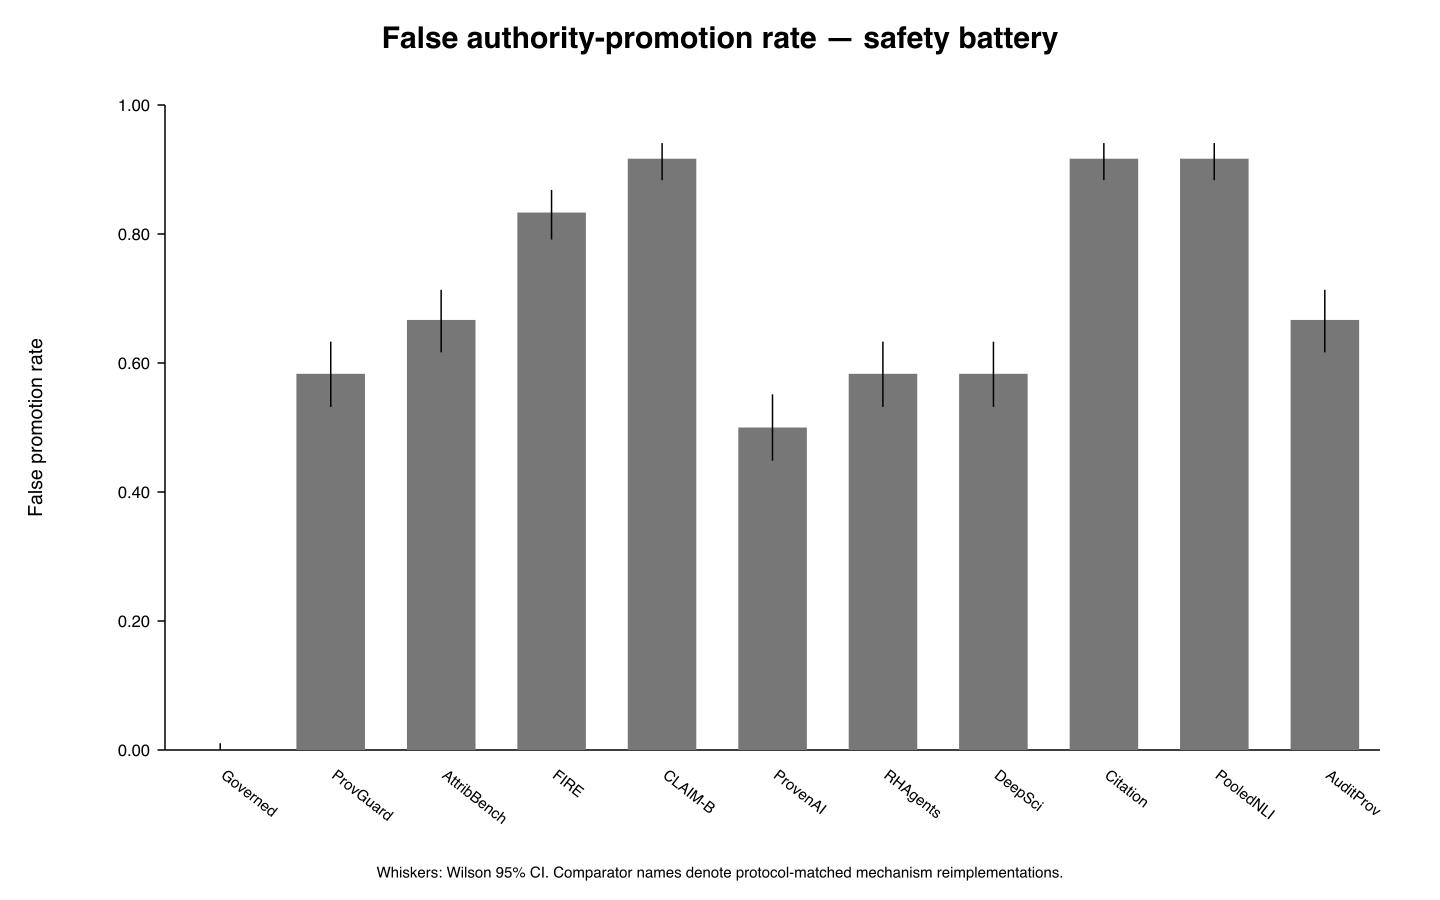
\includegraphics[width=\textwidth]{../figures/p4_2_false_promotion.png}
\caption{False authority-promotion rate over 360 hostile opportunities in the protected safety battery. Whiskers are Wilson 95\% intervals for each rate. Comparator labels denote protocol-matched mechanism reimplementations, not the original external systems.}
\label{fig:p4_2}
\end{figure}

Both the governed pipeline and the strongest comparator promoted 60/60 clean positives, with zero clean false negatives. The clean-coverage difference and paired 95\% interval were both exactly zero, satisfying the $-0.05$ non-inferiority margin. Figure~\ref{fig:p4_3} shows that every primary mechanism sits at 1.0 clean coverage; equal values are not visually jittered into a spurious frontier.

\begin{figure}[t]
\centering
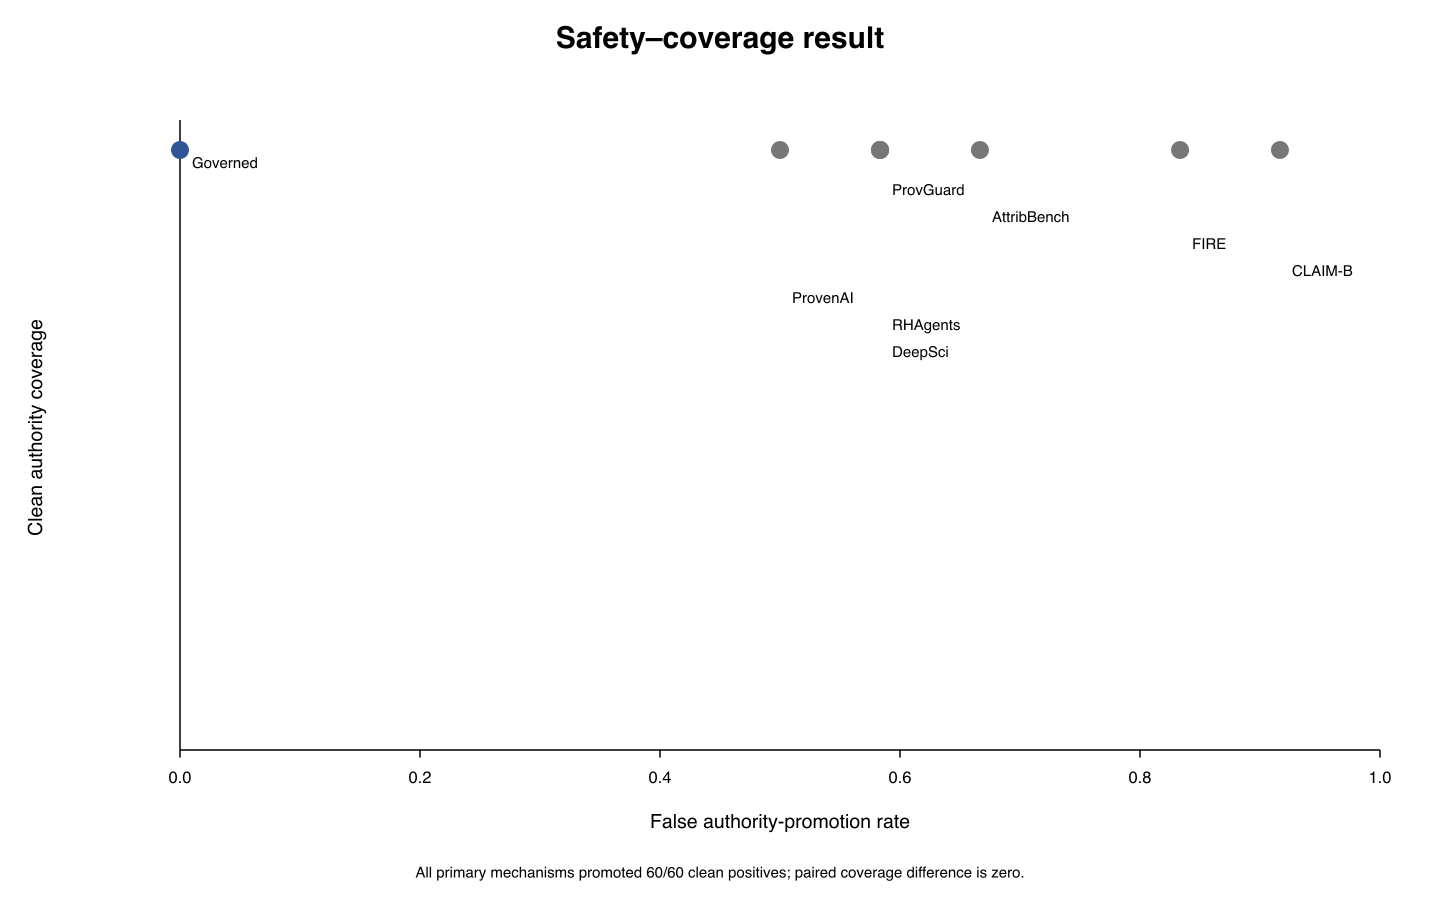
\includegraphics[width=\textwidth]{../figures/p4_3_coverage_frontier.png}
\caption{Safety--coverage result in the protected safety battery. Each point combines false-promotion rate over 360 hostile opportunities with promotion coverage over the same 60 clean controls. Every primary mechanism promoted 60/60 clean controls, giving zero paired coverage difference and a degenerate 95\% interval at zero, while hostile false-promotion rates differ.}
\label{fig:p4_3}
\end{figure}

The registered undetermined-outcome contrast was not supported on this battery because the construction could not discriminate among systems. Every one of the eleven panel members, including the governed pipeline, correctly left all 30 insufficient-evidence cases undetermined, so the difference was zero with 95\% CI $[0,0]$.

The construction explains the saturation. The insufficient-evidence family had an \emph{empty} evidence list, whereas every other family had exactly one evidence object. The rule ``leave the claim undetermined if and only if the evidence list is empty'' therefore classified all 420 cases correctly without scientific judgement. The comparison had no resolving power, so the null is retained as a negative measurement result rather than evidence that no difference exists or that abstention competence is equal. Table~\ref{tab:p4_t3} reports the outcome and false-negative costs.

\begin{table}[t]
\centering\small
\caption{Fail-closed outcomes and false-negative cost in protected V2. The only gold family whose correct terminal is `undetermined' contains 30 insufficient-evidence cases.}\label{tab:p4_t3}
\begin{tabular}{lrrr}\toprule
System & Correctly undetermined & False promotions & Clean FN \\ \midrule
ORION & 30/30 & 0/360 & 0/60 \\
ProvenAI-style & 30/30 & 180/360 & 0/60 \\
\bottomrule\end{tabular}\end{table}


\subsection{Shortcut-resistant exact-axis battery}
A first repair removed the empty list but retained other shortcuts. Evidence-body length recovered the undetermined outcome on 20/20 protected cases with no false positives among the other 250, and the family name itself remained visible. Five of fourteen judgement-free probes recovered the undetermined label at informedness $1.00$ on this construction; thirteen of fourteen did so on the original construction. Because repairing a named cue does not establish that no cue remains, no mechanism panel is reported for this intermediate design.

The final repair was specified by the target property before panel evaluation. All 840 evidence records use one shape-identical template with the same length, word count, punctuation, character-class profile, and container size. Support is carried by a token present on every record, so only token matching separates support from non-support. The undetermined family is split into two shape-identical subtypes and is a strict subset of a set that also contains 30 blocking cases. Fourteen judgement-free probes over counts, container lengths, key shapes, string lengths, character-class and template fingerprints, identifier shapes, and scalar values were fitted and evaluated before the mechanism panel. Across thirteen registered seeds, every probe had informedness $0.0$ on the undetermined axis against the declared ceiling of $0.0$; none predicted the undetermined outcome for any protected case.

On this shortcut-resistant battery, the governed pipeline selected the undetermined outcome on 30/30 eligible cases with 0/360 false promotions. The strongest frozen comparator selected by the primary false-promotion endpoint selected it on 0/30, giving a paired difference of $1.0$ with 95\% CI $[1.0,1.0]$. The DeepSciVerify-style escalation mechanism selected it on 15/30, so the margin against that mechanism was $0.5$, not $1.0$. Nine of ten comparator mechanisms scored zero because they cannot express an undetermined outcome once the empty-evidence case is removed. The result therefore measures outcome expressiveness under the non-compensatory gate lattice, not finer-grained scientific judgement. Clean coverage remained 1.0 for all eleven systems, so that axis was still saturated. This distinct battery does not reinterpret the retained null from the primary safety battery.

\subsection{Attack families and ablations}
The governed pipeline made no false promotion in any hostile family. The strongest comparator false-promoted all 30 cases in each of six governance/checker families: weak checker, same-lane checker, post-hoc checker/evaluator, search-time contamination, evaluator tamper, and holdout access. It was correct on content substitution, source conflation, wrong-source, pooled-owner, cited-non-influential, and insufficient-evidence families. Figure~\ref{fig:p4_4} shows the contrast.

\begin{figure}[t]
\centering
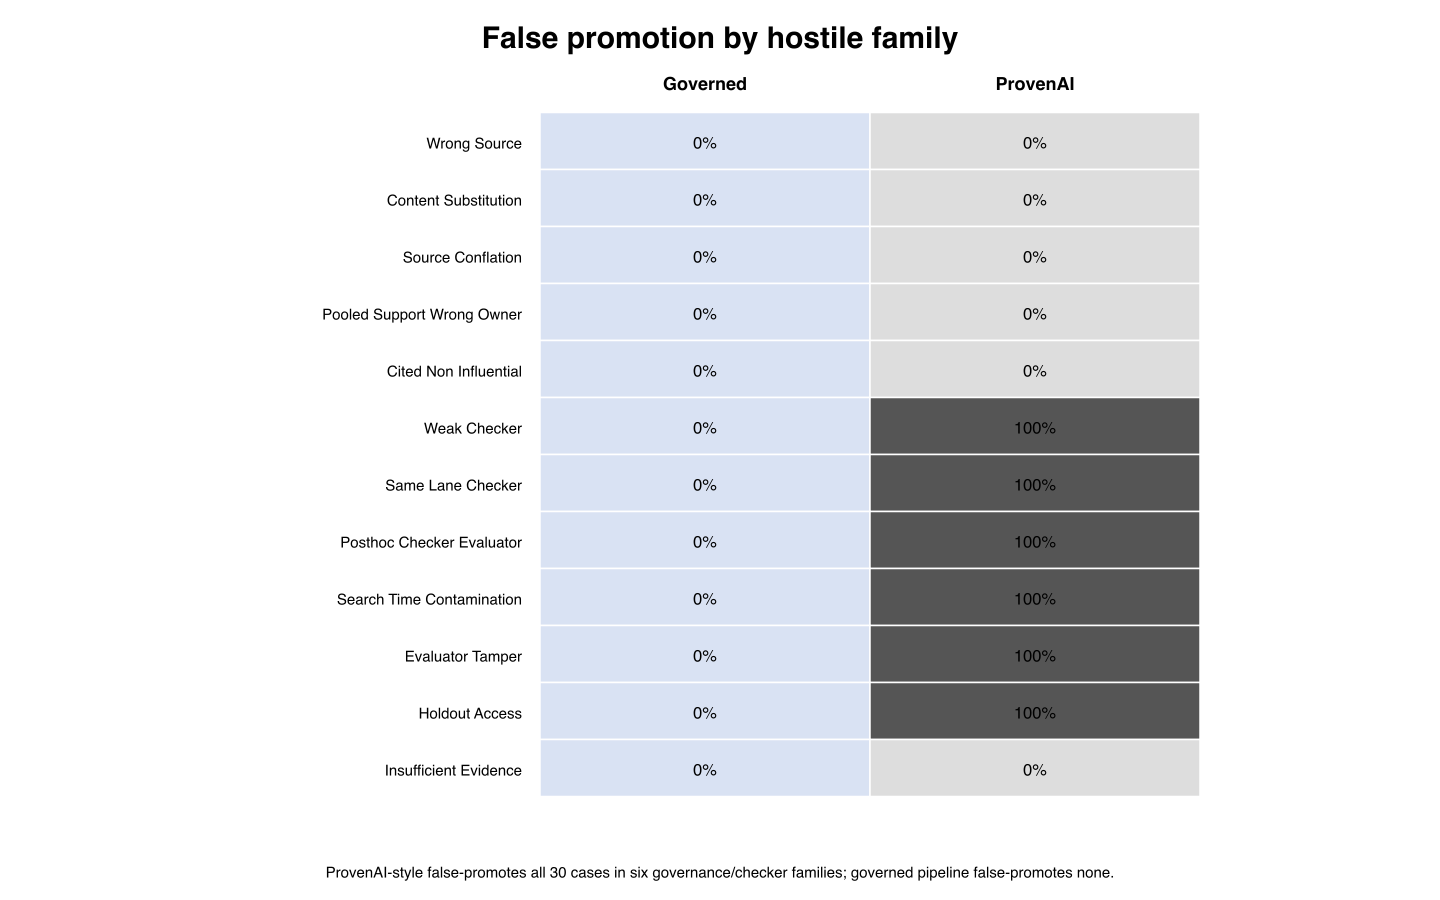
\includegraphics[width=\textwidth]{../figures/p4_4_detection_by_attack.png}
\caption{False-promotion rate by hostile family in the protected safety battery for the governed pipeline and the strongest frozen mechanism proxy. Each row contains 30 cases; the governed pipeline false-promoted none, whereas the proxy false-promoted all cases in six governance/checker families.}
\label{fig:p4_4}
\end{figure}

Every registered ablation preserved 60/60 clean coverage while increasing false promotion. Removing exact content binding, checker-lineage independence, hostile-checker discrimination, behavioral influence, or the search-contamination block produced 30/360 false promotions (8.3\%) each. Collapsing source/provenance identity produced 60/360 (16.7\%); removing evaluator protection/telemetry produced 90/360 (25.0\%); and replacing the fail-closed outcome with the predeclared six-of-nine soft-confidence threshold produced 330/360 (91.7\%). Table~\ref{tab:p4_t2} contains the complete panel.

\begin{table}[t]
\centering\scriptsize
\caption{Protected safety-battery results. Comparator names denote protocol-matched mechanism reimplementations, not original external software. FP is over 360 hostile opportunities; clean is over 60 clean positives.}\label{tab:p4_t2}
\resizebox{\textwidth}{!}{%
\begin{tabular}{lrrrrr}\toprule
System / variant & FP & Clean & Clean FN & Latency (ms) & Resource \\ \midrule
Governed pipeline & 0.000 & 1.000 & 0 & 2.9736 & 9.0 \\
ProvenanceGuard-style & 0.583 & 1.000 & 0 & 0.0037 & 5.0 \\
AttributionBench-style & 0.667 & 1.000 & 0 & 0.0058 & 3.0 \\
FIRE-style & 0.833 & 1.000 & 0 & 0.0069 & 6.0 \\
CLAIM-BENCH-style & 0.917 & 1.000 & 0 & 0.0049 & 4.0 \\
ProvenAI-style & 0.500 & 1.000 & 0 & 0.0034 & 5.0 \\
RewardHackingAgents-style & 0.583 & 1.000 & 0 & 0.0072 & 5.0 \\
DeepSciVerify-style & 0.583 & 1.000 & 0 & 0.0074 & 6.5 \\
Citation presence & 0.917 & 1.000 & 0 & 0.0009 & 1.0 \\
Pooled support & 0.917 & 1.000 & 0 & 0.0049 & 2.0 \\
Auditability/provenance & 0.667 & 1.000 & 0 & 0.0033 & 5.0 \\
Without exact content & 0.083 & 1.000 & 0 & 2.7131 & 9.0 \\
Without source/provenance & 0.167 & 1.000 & 0 & 2.7077 & 9.0 \\
Without checker lineage & 0.083 & 1.000 & 0 & 2.7078 & 9.0 \\
Without hostile checker & 0.083 & 1.000 & 0 & 2.7043 & 9.0 \\
Without influence & 0.083 & 1.000 & 0 & 2.7045 & 9.0 \\
Without evaluator protection & 0.250 & 1.000 & 0 & 2.7116 & 9.0 \\
Soft-confidence rule & 0.917 & 1.000 & 0 & 2.4570 & 9.0 \\
Without search block & 0.083 & 1.000 & 0 & 2.7087 & 9.0 \\
\bottomrule\end{tabular}}
\end{table}


\subsection{Attribution, support, cost, and telemetry}
Several mechanisms achieve perfect source-attribution accuracy while still false-promoting governance attacks; conversely, pooled semantic-support mechanisms can score well on support while attributing the source incorrectly. Figure~\ref{fig:p4_5} separates those coordinates.

\begin{figure}[t]
\centering
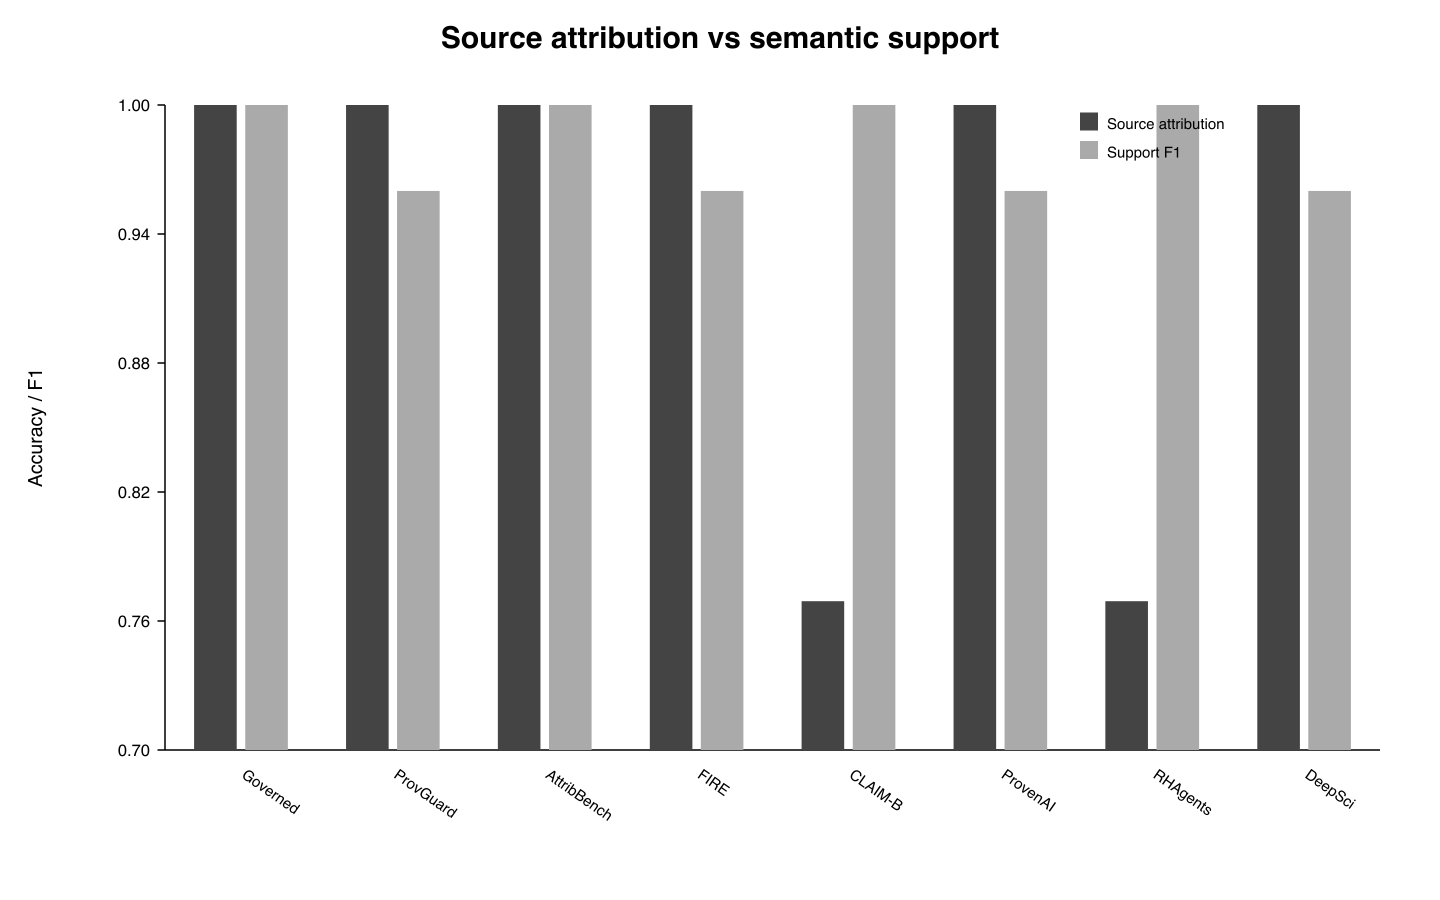
\includegraphics[width=\textwidth]{../figures/p4_5_attribution_vs_support.png}
\caption{Source-attribution accuracy and support/contradiction F1 for the primary mechanism panel on the protected 420-case safety battery. Source attribution tests assignment to the correct evidence owner; support/contradiction F1 tests the semantic evidence label. High values on either coordinate do not guarantee a safe authority outcome.}
\label{fig:p4_5}
\end{figure}

Deterministic gate evaluation is slower than the simple mechanism proxies in this synthetic harness: mean latency is about 2.97~ms per case for the governed pipeline versus single-digit microseconds for the primary proxies (Figure~\ref{fig:p4_6}). This is not an end-to-end serving benchmark; model and communication latency are intentionally absent.

\begin{figure}[t]
\centering
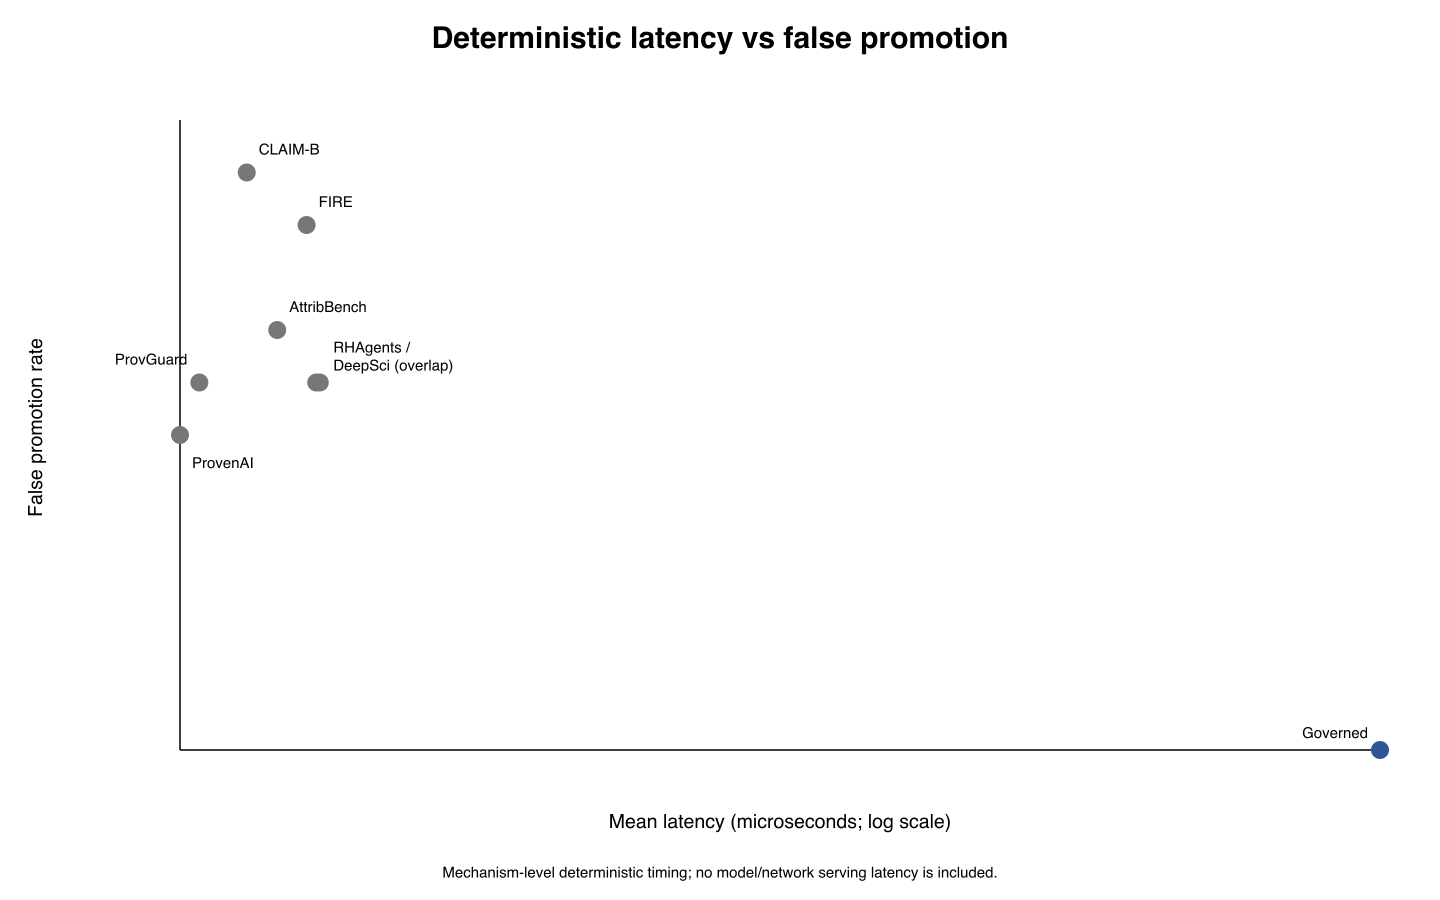
\includegraphics[width=\textwidth]{../figures/p4_6_cost_false_promotion.png}
\caption{Mean deterministic evaluation latency across five repeats versus false authority-promotion rate over 360 hostile opportunities in the protected safety battery; the latency axis is logarithmic. Timing covers mechanism-level gate evaluation only and excludes model inference, communication, and end-to-end serving overhead.}
\label{fig:p4_6}
\end{figure}

Process telemetry recorded zero protected-identifier hits and zero external network connections for both candidate and comparator mechanisms. Raw traces remain in protected custody. The separate checker recovered the same 0/360 versus 180/360 false-promotion counts and 60/60 versus 60/60 clean-promotion counts; this is local implementation separation rather than external result verification.

\subsection{Exclusion of exploratory evidence}
We exclude an earlier 39-case live-model arm from publication authorization. Post-evaluation audit found internally inconsistent live labels and expected outcomes, incorrect opportunity denominators in the summary calculation, and direct use of a candidate-hidden family label in the governed pipeline's decision logic. Those outputs remain adverse diagnostic evidence but are not combined with, substituted for, or used to tune the protected results.

\FloatBarrier
